\question
Describe the three main kinds of $\beta$-decay, and the kinematic conditions under which each occurs.   At fixed mass number, $A$, how many isotopes are typically stable with respect to $\beta$-decay and why?\marks{4}
\ANS{

[THIS QUESTION IS ENTIRELY BOOKWORK]


(i)

$\beta^-$: $n\rightarrow p+e^-+\bar \nu_e$ or ${}^A_Z X \rightarrow {}^A_{Z+1}Y + e^-+\bar\nu_e$ needs nuclear masses $m_X>m_Y+m_e+m_\nu$.

$\beta^+$: $p\rightarrow n+e^++\nu_e$ or ${}^A_Z X \rightarrow {}^A_{Z-1}Y + e^-+\bar\nu_e$ needs nuclear masses $m_X>m_Y+m_e+m_\nu$.

$e$-capture: $p+e^-\rightarrow n+ \nu_e$ or ${}^A_Z X + e^- \rightarrow {}^A_{Z-1}Y +\nu_e$ needs nuclear masses $m_X+m_e>m_Y+m_\nu$.

(ii)
Then need a short description of the main points given by this slide from lectures:
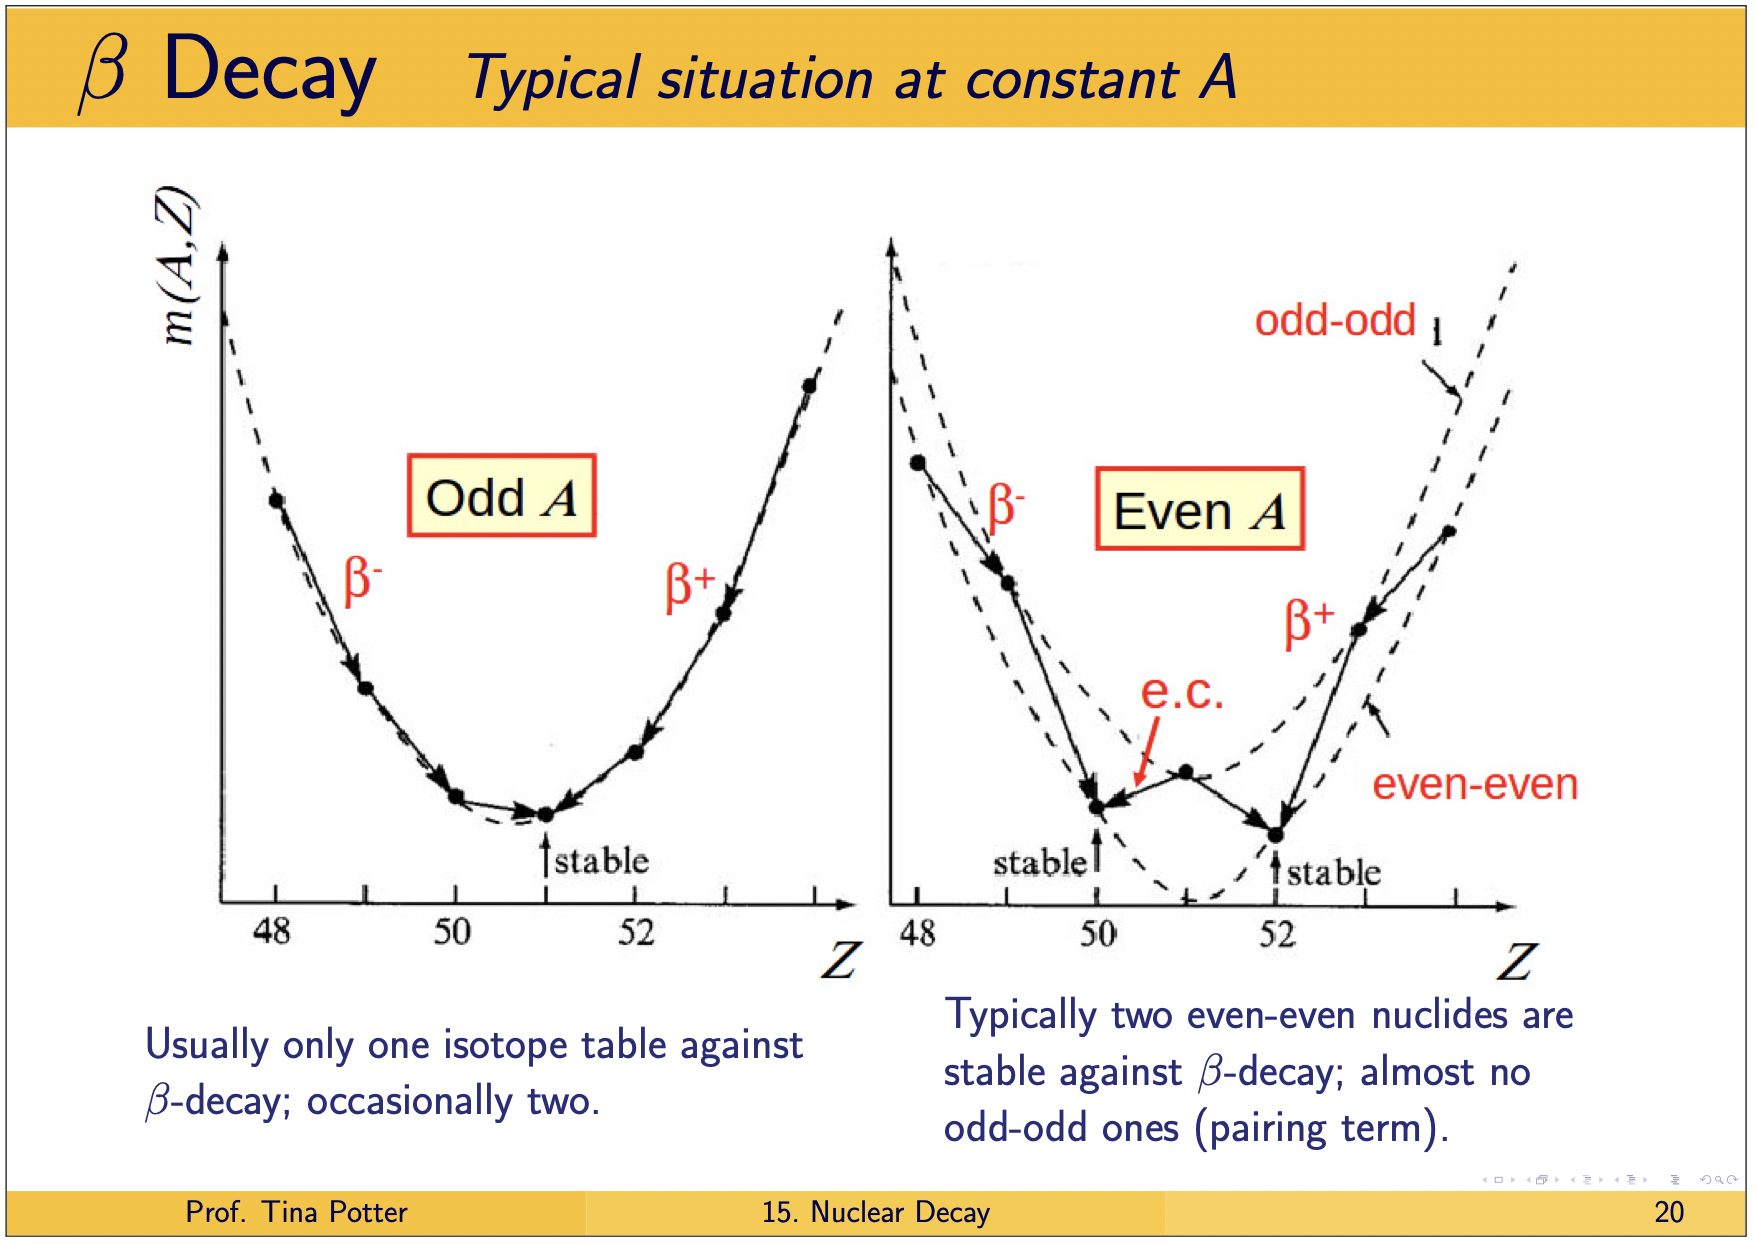
\includegraphics[width=0.8\textwidth]{Images/potter_nuclear_slide_20.png}.
}
\question
Describe the principles underpinning radio-carbon dating.\marks{4}
\ANS{

[THIS QUESTION IS ENTIRELY BOOKWORK]

(1) 14N+n to 14C+p in upper atmosphere due to cosmic rays, (2) leads to one part in $10^{12}$ of ${}^{14}$C in atmos, (3) uptake by living organisms until their death, (4) ${}^{14}$C $\rightarrow$ ${}^{14}$N+e+nubar with half life of 5730 years, so (5) measure num decays per second per unit mass (specific decay rate) to infer age since death.  

Lectures noted:
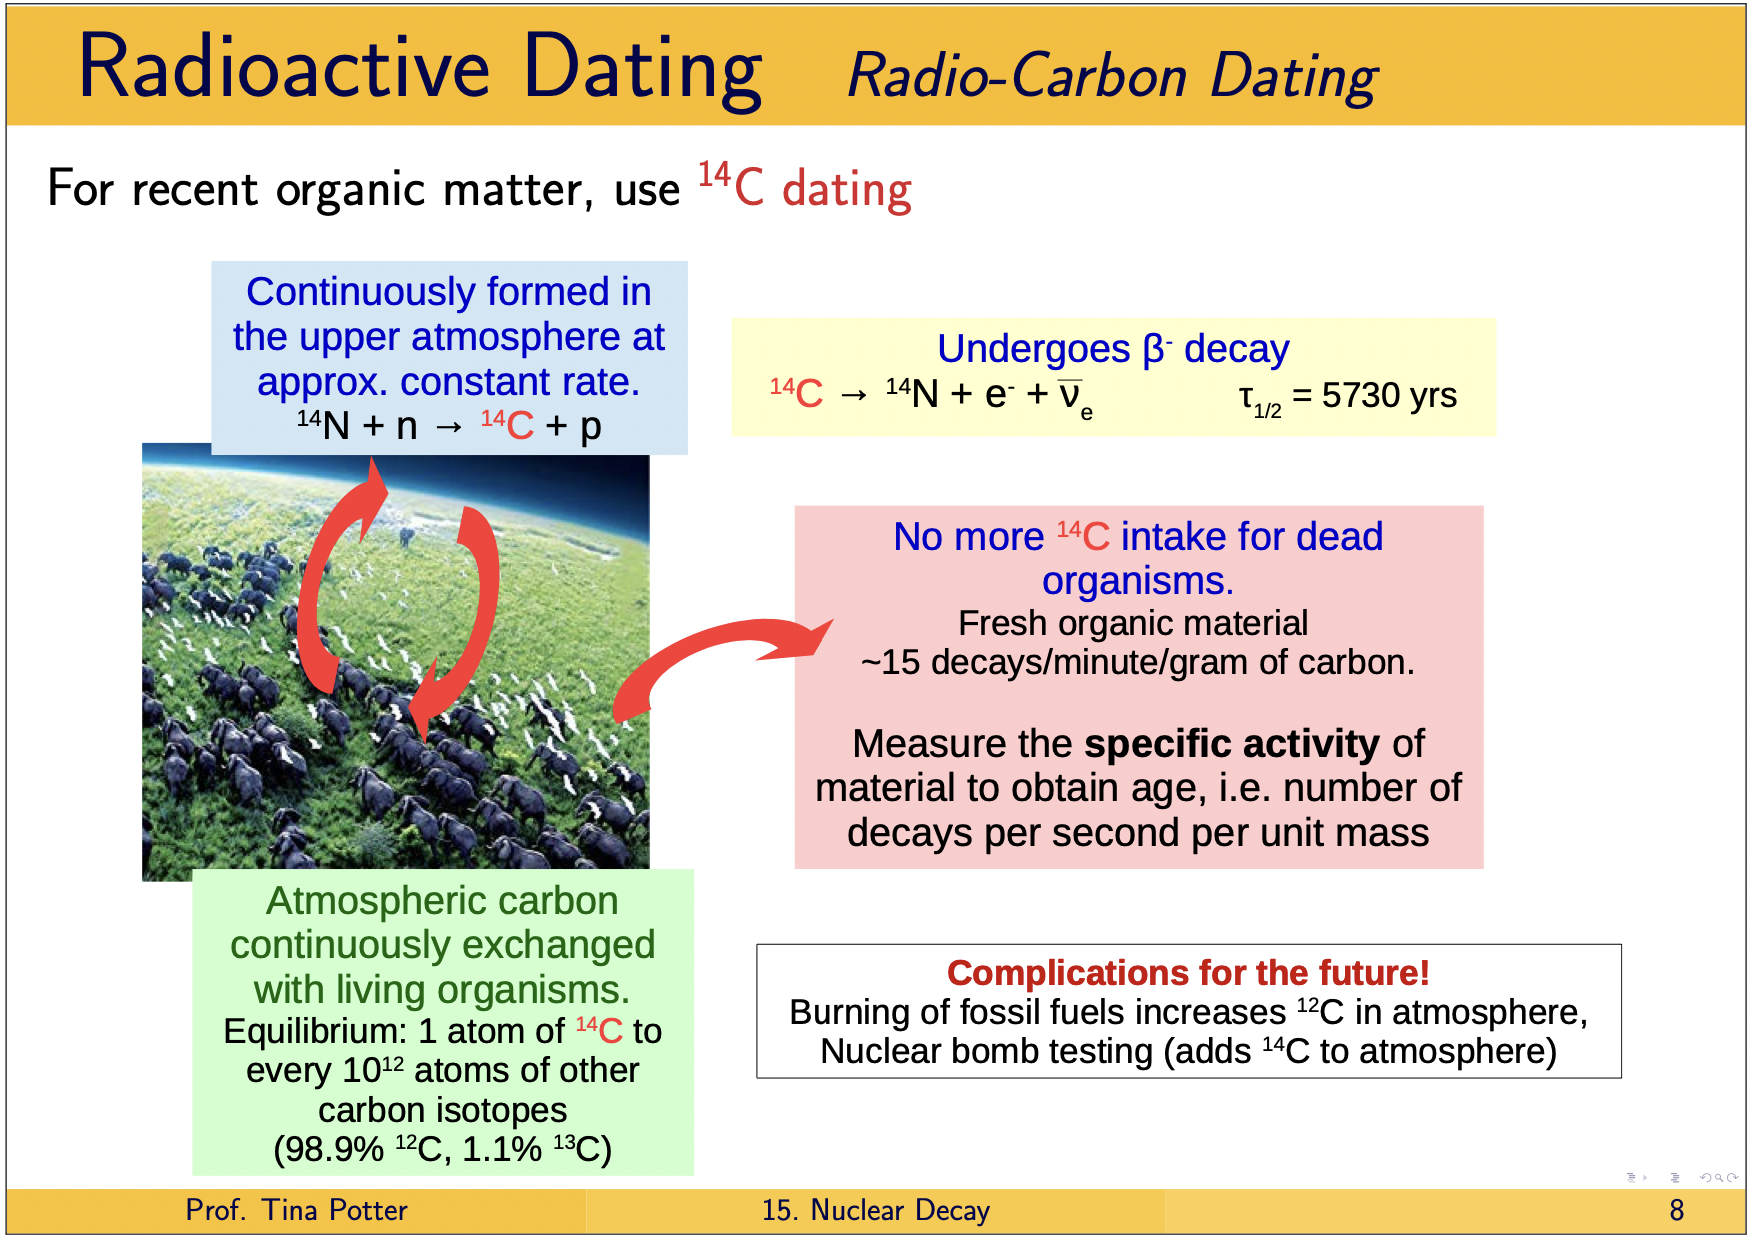
\includegraphics[width=0.8\textwidth]{Images/potter_nuclear_slide_8.png}.
}
\question


The Standard Model has four gauge bosons:  $g$, $W$, $Z$ and $\gamma$.  The  Feynman rules of this theory include fundamental vertices which couple together \textbf{only} certain groups of these gauge bosons.  A fundamental vertex of The Standard Model coupling together $N$ gauge bosons (i.e., one having $N$ legs) is called an `$N$-gauge-boson vertex'.
\begin{parts}
\part
How many two-gauge-boson vertices exist in The Standard Model? Draw a picture of each vertex, clearly indicating the type of boson on each leg.
\part
Repeat (a) for three-gauge-boson vertices.
\part
Repeat (a) for four-gauge-boson vertices.
\part
Repeat (a) for five-gauge-boson vertices.
\end{parts}\marks{4}
 
\ANS{
\clearpage

COMMENT ON QUESTION:

This is not supposed to be bookwork `as such' (though it is related) since the way SM vertices are talked about in both this course and in many books is usually very compartmentalised. That is to say that QED vertices will be usually be talked about in one part of the course, and weak vertices in another, etc.  Although every book/lecturer will almost certainly say somewhere that `photons couple only to electric charge' or that `gluons couple only to colour',  it is very rare for a lecturer or a text book to explicitly make a statement like `there is no $g\gamma\gamma$-vertex'. The students should be able to see there is not one (if they don't already know this), but from past experience supervising students in this course I suspect many will not. Similarly, many students seem to have a very vague idea about which gauge-boson self interactions area allowed -- or for that matter whether they are constrained at all.  The point of this question, therefore, is to take the vertices of the SM outside the friendly context of individual sub-theories (like QCD or QCD) and put them into a wider context, so that we can then determine which of the students have (or don't have) a clear/firm idea that there is no $ggZ$-vertex, etc.   The somewhat wordy construction used in the question is there (rather than a free form `just tell me about the vertices which do exist') to make sure that the people answering the question have in mind the full generality of what they are being asked to consider. and can give large answers if they want to. [The brightest of them will, however, rapidly realise that there is very little to do in this question -- which is fine.]
 
 \vspace{1cm}
 
 ANSWER TO QUESTION:
 
 (a)
 There are 0 two-gauge boson interactions in the SM.

 (b)
 There are 3 three-gauge boson interactions in the SM.  The gauge bosons on the legs of each in turn are:
 
1: $ g g g $, 
 
2:  $ W W Z $, 
 
3: $ W W \gamma $.
 
  
 (c)
 There are 5 four-gauge boson interactions in the SM.  The gauge bosons on the legs of each in turn are:
 
 1: $ g g g g $, 
   
2:  $ W W W W $, 
 
3:  $ W W Z Z $, 
 
4:  $ W W Z \gamma $, 
 
5:  $ W W \gamma \gamma $.
 
 (d)
 There are 0 five-gauge boson interactions in the SM.
 }
